\documentclass[a4paper,14pt]{extarticle}

%%%%%%%%%%%%
% Preamble

% The most important
\usepackage{examstylo}
%%% Provides the following:
%% For typesetting
% \mrm{} % shorthand mathrm
% \thus % Implication symbol
% \sm % small minus (for \sm2 - 2 = \sm 4)
% \meuro % neat euro sign
% \deg % degree
% \mli{} % multiletter identifier (prevents linebreak)
% \cldots % compact \ldots
% \oldots % orange compact \ldots (like in Kern)
% \rom{} % roman numeral
% \intextbullet % Make a bulletpoint
% \lognl[base] % make a logarithm base base
% \deriv{y}{x} % make total derivative dy/dx
%
%% For control
% \comment{} comment everything inside
% 
%% And some colors
% \red{}
% \blue{}
% \orange{} % Like in Kern

%%% Some notes:
% \newsubquestion{}{} works with package paracol to make two columns. if you want a newline after the subquestion, put the \newline INSIDE the question txt (i.e., {example text\newline}) 
% use \begin{multicols}{2} for two-column subquestions. its not perfect but so arent you
  % It will force an empty line above (and below?) use \vspace{-\lineheight} to remedy
% Watch out with a \footnote: margin notes do not move with the text to the newpage after a footnote was inserted.
% You can use \insertemptypage to insert an empty page



%%%%% %%%%% Options!
%% Uncomment this to use points from Questions (ignored if use points from subquestions)
%\UsePointsFromQuestions % < This
%% Uncomment this to use points from SUBquestions
\UsePointsFromSubQuestions % < This
%% Uncomment this to make a full title page
%\MakeTheFullTitlePage % < This
%% Uncomment this to make a simple title on the first page (ignored if make full titlepage)
\MakeTheSimpleTitlePage % < This
%% Uncomment this to make the formula page
%\MakeTheFormulaPage % < This
%% Uncomment this to make the worksheets
%\MakeTheWorksheetPages % < This

%% Uncomment this to use Arial (Ugly!)
\UseArialFont % < This


%% Footer options
\SetFooterOptions[% Set options for the footer
  showleft=False,%=True
  showcenter=True,%=True
  showright=True,%=True
  ]{}

%% Exercise options
\SetExerciseOptions[% Set options for exercises
  PutExerciseOnNewPage=Fale,%=True to show every (except first) exercise on a new page
  PutFirstExerciseOnNewPage=False,%=True to have the first exercise on a new page
  firstexercisevskip=\baselineskip,%=\baselineskip if first exercise not on new page, how much vspace before?
  ]{}

%% Worksheet options
\SetWorksheetOptions[% Set options for exercises
  ShowTitle=False,%=True to show the title on the first page of the worksheets
  ]{}
  
%% Simple titlepage options
\SetSimpleTitleOptions[% Set options for exercises
  thestyle=Exerciselike,%=Default [Attempts to look like full titlepage, but small], =Exerciselike [Looks more like the exercise seperator]
  ]{}

  
%%%%% %%%%% BEGIN document
\begin{document}


%%%%% Title Page Settings
\title{Test for a test}
\extratitletext{{\Large Versie A}} % extra concise info e.g, {\Large Versie A}
%\leftfoottext{testtest-v0} % Text in the left box of the footer

\date{Zondag 09-02-1992}
%\time{09:02\enspace--\enspace16:20\,uur}

\noteforthelastpage{% Put text here to have a note on the last page
%\textbf{Credit:} Hello this is credit which is shown on the last page.
} % end text for lastpage note

%%% Put text for the title page Here
% Use \totqstns and \totpts to reference total questions and total points resp.
\titlepagetext{
Bij dit examen hoort een uitwerkbijlage. 

\vfill
Dit examen bestaat uit \totqstns\ vragen.\par
Voor dit examen zijn maximaal \totpts\ punten te behalen.\par
} % End of the title page text

%%% Put text here for the simple title on the first page
% Use \totqstns and \totpts to reference total questions and total points resp.
\simpletitletext{
\textit{Deze toets bestaat uit \totqstns\ vragen (\totpts\ punten).\\
Veel succes en plezier!\\
  }
}


% Make title pages if instructed to
\ifmakefulltitlepage
  \maketitlepage % inserts a \newpage
\else
  \ifmakesimpletitlepage
    \makesimpletitleonfirstpage % does not insert a \newpage
  \fi
\fi


\pagestyle{mainpagestyle} % Apply the main style
%%%%% Formula Page (?)

\formulapagetext{% Put text here for the formula page(s)


} % End of formula page text

% Make the formula page if instructed to
\ifmaketheformulapage
  \makeformulapage
\fi

%%%%% Begin With the Body
\makeatletter\ifOptExc@firstexconnewpage
  \setmainpagegeometry
\fi\makeatother

%%% New exercise
%\newexercise{Lorem} \label{exc:lorem}

%\begin{wrapfigure}[]{r}{0.3\textwidth} % Use for illustrations, not figures
%\begin{wrapfigure}[<number of lines>]{<capital for float>}{0.5\textwidth}
%\centering
%    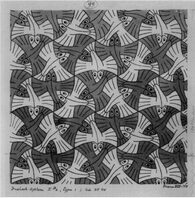
\includegraphics[width=0.25\textwidth]{escher.jpg}
% \caption{}
%\end{wrapfigure}



\newquestion[3]{\label{q:vraagX}quis nostrud exercitation ullamco laboris nisi ut aliquip ex ea commodo consequat. ea commodo consequat.} 
\newsubquestion[2]{No sabía, de tristezas, ni de lágrimas, Ni nada, que me hicieran llorar,}
\newsubquestion[2]{Yo sabía de cariño, de ternura. Porque a mí desde pequeño Eso me enseño mamá,}
\newsubquestion[2]{eso me enseño mamá Eso y muchas cosas más.}
\newsubquestion[2]{Yo jamás sufrí, yo jamás lloré. Yo era muy feliz, yo vivía muy bien\newline}

\showpoints
\newquestion[3]{\label{q:vraagXX}quis nostrud exercitation ullamco laboris nisi ut aliquip ex ea commodo consequat. En quaestio~\ref{q:vraagXXX} habes responsum.\newline} 


\newquestion[3]{\label{q:vraagXXX}quis nostrud exercitation ullamco laboris nisi ut aliquip ex ea commodo consequat. ea commodo consequat.}\vspace{-\lineheight}%\vspace{-0.83333\baselineskip}  
\begin{multicols}{2}%
\newsubquestion[2]{$y=x^2-3$}
\newsubquestion[2]{$L=4\pi R^2 \sigma T^4$}
%\newsubquestion[2]{$y=x^2-3$}
\newsubquestion[2]{\label{sq:subq}Yo jamás sufrí, yo jamás lloré. Yo era muy feliz, yo vivía muy bien}
\columnbreak% Notice the columnbreak
\newsubquestion[2]{$y=x^2-3$}
\newsubquestion[2]{$y=x^2-3$}
\newsubquestion[2]{$y=x^2-3$}
\end{multicols}



%%% This is the end (do not touch)
\lastpageofthetest\
%%

%%%%% HERE STARTS THE WORKSHEETS
\worksheetcontent{ % Put content here for the worksheets
                   % Use \refquestion{<label>} to refer to a question
\refquestion{q:vraag}\newline
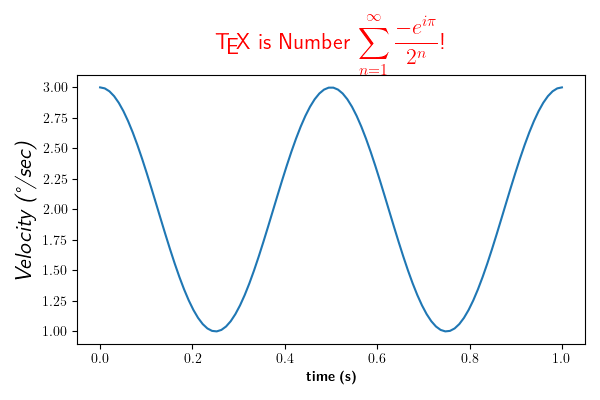
\includegraphics[width=0.8\textwidth]{random_graph.png}

\vfill

\refquestion{q:vraagvier}\newline
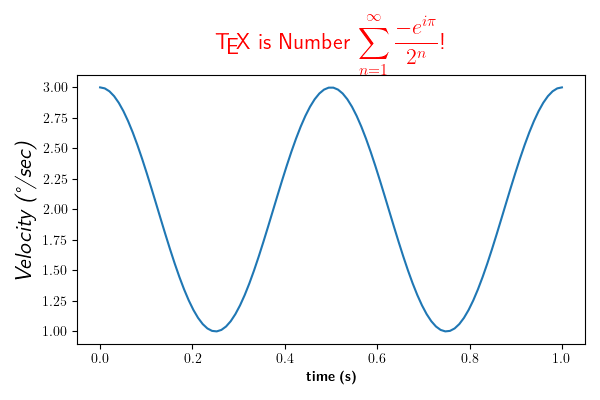
\includegraphics[width=0.8\textwidth]{random_graph.png}

\newpage

\refquestion{q:vraagvijf} en \refquestion{q:vraagzes}\newline
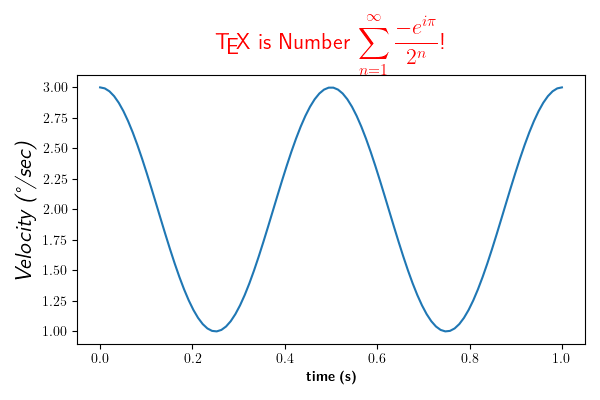
\includegraphics[angle=90,width=0.8\textwidth]{random_graph.png} % Sidenote: The rotating package introduces a sidewaysfigure

} % End worksheet content

% Make the worksheet pages if instructed to
\ifmakeworksheetpages
  \makeworksheets
\fi



\end{document}
